\documentclass[a4paper]{article}
\usepackage{graphicx}
\usepackage{hyperref}
\usepackage{authblk}
\usepackage{multirow}
\usepackage{booktabs}
\usepackage{array}

\title{Semi-automatic staging area for high-quality structured data extraction from scientific literature}
\author[1,2]{Luca Foppiano}
\author[1]{Tomoya Mato}
\author[3]{Kensei Terashima}
\author[4]{Pedro Ortiz Suarez}
\author[3]{Taku Tou}
\author[3]{Chikako Sakai}
\author[3]{Wei-Sheng Wang}
\author[2]{Toshiyuki Amagasa}
\author[3]{Yoshihiko Takano}
\author[1]{Masashi Ishii}
\affil[1]{Materials Modelling Group, Data-driven Materials Research Field, Centre for Basic Research on Materials, NIMS, Japan}
\affil[2]{Knowledge and Data Engineering, Centre for Computational Sciences, University of Tsukuba, Japan}
\affil[3]{Frontier Superconducting Materials Group, MANA, NIMS, Tsukuba, Japan}
\affil[4]{DFKI GmbH, Germany}

\begin{document}

\maketitle

\begin{abstract}
    TBA
\end{abstract}

\section{Introduction}

The emergence of new methodologies using machine learning for materials exploration has given rise to a growing research area called materials informatics (MI) ~\cite{10.3389/fchem.2022.930369}.
This field leverages the knowledge of the materials data accumulated in the past to efficiently screen candidates of the materials with desired properties.
As a matter of course, such an approach requires a larger number of material-related data for training models.
Researchers have been developing large aggregated databases of physical properties generated by first-principles calculations based on Density Functional Theory (DFT), such as Materials Project~\cite{materialsprojectJain2013}, JARVIS~\cite{aflowcurtarolo2012aflow}, NOMAD~\cite{nomad}, that played a role of a strong driving force for the development of materials informatics. 
Using DFT data for machine learning (ML) in materials science has become popular since, in principle, it allows researchers to simulate and obtain various types of physical properties of the target materials only by knowing the crystal structures of the subjects. 
Those DFT codes are designed so that they reproduce/simulate the physical properties that should be observed by experiment in reality. 
Nonetheless, caution must be exercised while utilising these computed figures for constructing ML models aimed at steering experiments. This caution arises due to the potential lack of validity in their predictions when dealing with specific simplifications of the interactions between atoms and electrons in solids, such as electron-electron Coulomb correlation, spin-orbit coupling, and similar factors.

Au contraire, accumulated datasets of experimental data from scientific publications are still scarce, despite abundant availability of publications, and exponential growth in materials science~\cite{Pratheepan_2019}.
Currently, only a few limited resources exist, such as the Pauling File~\cite{Blokhin2018ThePF_paulingFile} and SuperCon~\cite{SuperCon}, necessitating reliance on manual extraction methods. 
This scarcity can be attributed to inadequate infrastructure and a shortage of expertise in the field.

% The lack of adequate infrastructure and expertise could have led to the creation of a single manual procedure that can extract information from diverse sources like plots, tables, and text all at once. However, while this approach may be viable in the short term, its sustainability diminishes over time. 
% On the other hand, constructing an automated process to accomplish this task presents many challenges. In the case of scientific publications, plots, tables, and text necessitates different treatments, and the resulting outputs must be merged and verified manually. Despite the challenges, it is possible to transition gradually towards automation by implementing iterative steps. This iterative approach involves reducing human involvement progressively while simultaneously optimising the efficiency of required human actions. 

SuperCon~\cite{SuperCon} was built manually from 1987~\cite{ishii2023structuring} by the National Institute for Materials Science (NIMS) in Japan and it is considered the gold standard in superconductors research.
Despite being praised for its excellent quality in numerous reports~\cite{roter2020predicting, stanev_machine_2017, tran2022machine, konno2021deep}, the updates of SuperCon have become increasingly challenging due to the high publication rate. 
However, in response to the need for a more efficient approach to sustain productivity, we embarked on the development of an automated system for extracting material and property information from the text contained in relevant scientific publications~\cite{lfoppiano2023automatic}. 
This automated process enabled the rapid creation of SuperCon\textsuperscript{2}, a comprehensive database of superconductors containing around 40000 entries, within an operational duration of just a few days. 
Matching the level of quality seen in SuperCon while simultaneously automating the extraction of organised data can be achieved with a properly designed curation process. 
We define as \emph{curation} the general term indicating the correction and validation of records in a database as a whole, and \emph{correction} as the specific process of modifying the values of one or more properties in a single record. 
At the moment of writing this article, we are not aware of any other curation tool focusing on structured databases of extracted information. 
There are several tools for data annotation, such as Inception~\cite{klie-etal-2018-inception}, and Doccano~\cite{doccano} which concentrate on text labelling and classification.

In this work we have designed a workflow along with a user interface crafted to simplify the curation procedure, encompassing the continuous and engaged oversight of data throughout its pertinent life cycle. 
This framework is custom-tailored to our superconductors database, yet it holds the potential for being adapted to alternative data frameworks.
We aim to produce structure data of a similar or superior quality to the one obtained by the classical manual method of reading PDF documents and noting information in an Excel file.

Our contributions to the field can be summarised as follows:
\begin{itemize}
    \item A user interface and a workflow acting on a machine-collected database. The interface exploits database navigation and an enhanced document viewer, similar to \cite{wang2022hammer}. We demonstrated our solution improves the quality of the curation as compared with the manual method (Section~\ref{sec:interface-evaluation}).
    \item We propose a mechanism that selects training data based on corrected records, and we demonstrate that such selections are rapidly improving the ML models (Section~\ref{subsec:training-data-generation-evaluation}).
    \item We devise an integrated anomaly detection process for the identification of outliers in the materials-properties database which results in a lower rejection rate (false positive rate) from domain-experts (Section~\ref{subsec:anomaly-detection-evaluation}).
\end{itemize}

The subsequent section (Section~\ref{sec:ingestion}) presents the data ingestion process.
Section~\ref{sec:curation-workflow} describes the curation workflow, and Section~\ref{sec:user-interface} the user interface on top of it.
Finally, we discuss our evaluation experiments in Section~\ref{sec:interface-evaluation}. 


\section{Ingestion process}
\label{sec:ingestion}

The ingestion process (Figure~\ref{fig:map-reduce}) is designed using an Extract-Aggregate approach we briefly introduced in our previous work~\cite{lfoppiano2023automatic}. 
In this section, we summarise the architecture (Section~\ref{sec:architecture}) and focus on the data transformation from the PDF document to the structured database (Section~\ref{subsec:data-formats}).

\begin{figure}[ht]
  \centering
  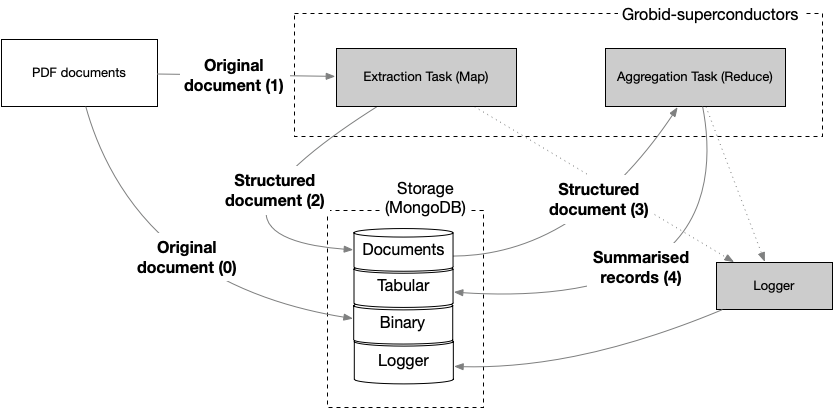
\includegraphics[width=\textwidth]{images/ingestion-schema.png} 
  \caption{Ingestion process}
  \label{fig:map-reduce}
\end{figure}

The "Extraction Task" takes as input PDF documents, stores them, and then processes them with Grobid-superconductors. 
Grobid-superconductors transforms the PDF documents into a rich representation document containing the original text and the extracted information in JSON format, which we will refer to as \textit{structured documents}.  
The "Aggregation Task" takes in input the \textit{structured document} and transforms it to a table format where each row contains one material, its T\textsubscript{c} and their related properties (we refer to as \textit{summarised record}, or, simply \textit{record}).

\subsection{Architecture}
\label{sec:architecture}

The two ingestion tasks are implemented in separate Python scripts that can run asynchronously either with a scheduler or using a publish-subscriber triggering mechanism. 
The storage is implemented using MongoDB\footnote{\url{https://www.mongodb.com}}, an open-source document database. 
We design the database in five collections: 
\begin{itemize}
    \item \textbf{binary}: contains the original PDF documents 
    \item \textbf{documents}: contains the \textit{structured documents}
    \item \textbf{tabular}: stores the \textit{summarised records}
    \item \textbf{logger}: contains information on the processing status of each document, including errors and status codes from the Grobid-superconductors API (Section~\ref{subsec:curation-and-processing-logs}).
    \item \textbf{training\_data} collects the raw information that can then be exported as training data (Section~\ref{subsec:feedback-loop-training-data})
\end{itemize}

We compute the unique signature for each original document by using the first 10 characters of the MD5 hash function on the binary content. 
We use this information to link the original document, the \textit{structured document} and the \textit{summarised records}.

\subsection{Data formats}
\label{subsec:data-formats}

The \textit{structured document} contains three main sections: a) bibliographic data (authors, DOI, title, publisher, journal, year of publication), b) runtime execution time from the server side (excluding the network and database delay), and c) a list of text passages, each representing a sentence.
Each passage is then composed of the following attributes (identified in orange in Figure~\ref{fig:data-flow-2}): 
\begin{itemize}
\item the text of the passage
\item the type of passage: sentence, or paragraph
\item the main section: body, header, or annex
\item the subsection within the section: title, abstract, paragraph, caption, etc.
\item the list of spans where each span represents one entity extracted from the text (in blue in Figure~\ref{fig:data-flow-2})
\item a list of layout tokens, which contains, for each token in the passage the layout information such as font size, font name, superscript, subscript, bold, and italic.
\end{itemize}

Each span aggregates a complex set of information illustrated in an example in Figure~\ref{fig:data-flow-2} and identified in blue:  links (in green), attributes (in red), PDF "boxes" coordinates (in yellow), and annotation reference to the sentence (in light blue). 
The general information is composed of a unique identifier (calculated on certain span attributes), the \textit{text} contains the value of the extracted entity (e.g. \textit{FeSe}), the entity type or class (e.g. \texttt{<material>}).
Furthermore,\textit{Linkable} indicate whether the span respects the criteria to be linked to other entities and \textit{source} the ML model from which the entity was extracted. 

The links (green) indicate linked entities and their type (in our example the material FeSe is linked to 13K of type \texttt{<tcValue>}. 
The type indicates the algorithm used for extracting the relation and the "targetId" indicates the unique id of the relation target span (13 K).

The attributes are stored as a key-value and contain additional information extracted by the subsequent models such as the Material Parser. For example, the chemical formula is stored both as a string and as structured composition (a list of elements and their amount in the formula), the material class, and so on.

The "PDF boxes coordinates" (yellow) are expressed as lists of objects containing page number, top-right and bottom-left coordinates\footnote{Details on coordinates is available in the official grobid documentation \url{https://grobid.readthedocs.io/en/latest/Coordinates-in-PDF/\#coordinates-in-teixml-results}}. This information is sufficient to draw a set of rectangles on the PDF document ("the boxes") that encapsulate groups of tokens belonging to each annotation. An example of the final result can be seen in Figure~\ref{fig:pdf-view}.

\begin{figure}[htbp]
  \centering
  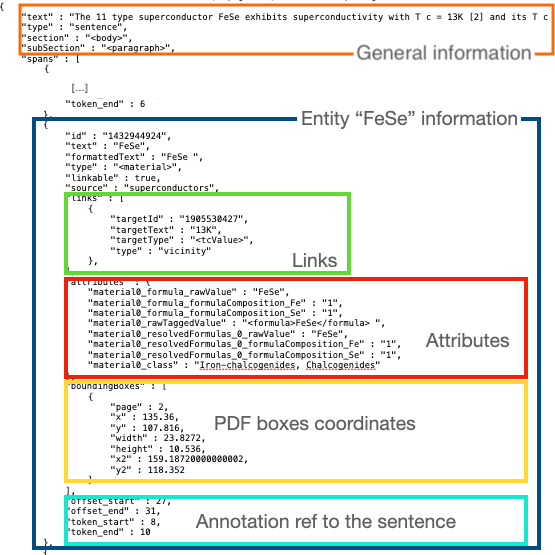
\includegraphics[width=1\textwidth]{images/data-flow-2} 
  \caption{Example of span encoding information of the extracted material \textit{FeSe}}
  \label{fig:data-flow-2}
\end{figure}

The "Aggregation Task" transforms the "structured document" in input to a tabular format comprising as many rows as the extracted materials records. 
Each column of the table represents the related information and properties. 
We format each record in JSON format required by MongoDb as illustrated in Figure~\ref{fig:data-flow-3}.

\begin{figure}[ht]
  \centering\small
  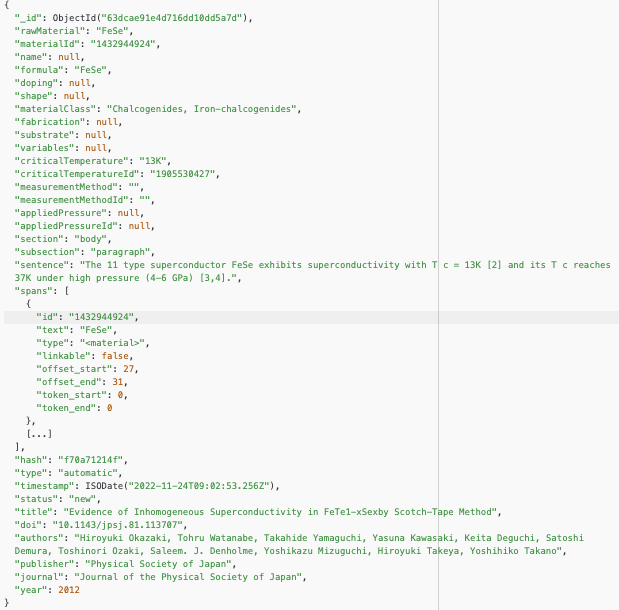
\includegraphics[width=1\textwidth]{images/data-flow-3} 
  \caption{Example of the aggregated record corresponding to the \textit{FeSe} material.}
  \label{fig:data-flow-3}
\end{figure}

The aggregation pivots around the relation materials-Tc and then attaches additional elements to it. 
A detailed description of the main fields can be found in our previous work~\cite{lfoppiano2023automatic}. The span objects corresponding to the entities linked together are repeated in this structure and are used to visualise the passage decorated with the extracted entities in this record.

For complex material names corresponding to multiple entities are split and stored in several records.
For example, a material name containing substitution variables like M Fe O (M=La, Cu) will result in two records having materials such as "La Fe O" and "Cu Fe O", respectively. 
In many other cases inferring the correct interpretation is left to curators. 
For example, the expression "Zn and Cu doping La Fe B" possibly has two meanings. Namely, it means LaFeB doped with both Zn and Cu at the same time, or LaFeB doped with Zn, and LaFeB doped with Cu. 

\section{Curation workflow}
\label{sec:curation-workflow}

% Once a structured database is collected, its data can be visualised and curated by domain experts. 
The curation process can be delineated as a structured workflow, wherein each record undergoes a series of transitions between distinct states. 
These transitions are determined by the actions that are executed on the record, encompassing various stages of refinement and enhancement. 
Figure~\ref{fig:curation-workflow} illustrate the concept in detail.
A record enters the workflow at the ingestion process (Section~\ref{sec:ingestion}) and its state can change by manual action or automatic process. 
In this workflow, the automatic process is "anomaly detection" (Section~\ref{subsec:anomaly-detection}) which aims to automatically mark outliers. 
There are four types of manual actions: 
\begin{itemize}
    \item \textbf{mark as valid}: when a record is considered corrected, without the need for any correction, 
    \item \textbf{mark as invalid}: the record is considered potentially invalid
    \item \textbf{remove}: the record is considered invalid
    \item \textbf{manual correction}: the record is updated 
    \item \textbf{reset}: the statuses previously changed (e.g. marked as valid or invalid) are reset
\end{itemize}.

Given an action that updates a field in a record, we define the \emph{original record} as the record \textbf{before the modification}, and the \emph{updated record} as the new record \textbf{after the modification}. 
The record data is persisted in every state of the workflow: in case of modifications both the "original" and "updated" records are kept and the "original" record is hidden in the user interface.  
Similarly, when a record is removed the data is kept but the record is hidden, while records marked as valid or invalid are kept visible. 
Such an approach is justified by the need to generate the history of each record over time (Section~\ref{subsec:curation-and-processing-logs}) and support the implementation of the undo/redo functionality if needed in future. 

The workflow establishes also that when a record is manually corrected, the raw data from which the record has been extracted, are collected as training data. This policy is indicated as "(*)" in Figure~\ref{fig:curation-workflow} and is described in detail in Section~\ref{subsec:feedback-loop-training-data}.

\subsection{Workflow control}
\label{subsec:workflow-control}

The action performed on the record combined with the curation status determines the next stage of the workflow. 
The curation status characterises each state in the workflow and is encoded by a combination of two fields: \emph{type}, and \emph{status} described in Section~\ref{subsec:curation-status}.
In addition, when a record is corrected we collect details regarding the type of error, and this process is described in Section~\ref{subsec:error-types}).

\begin{figure}[ht]
  \centering
  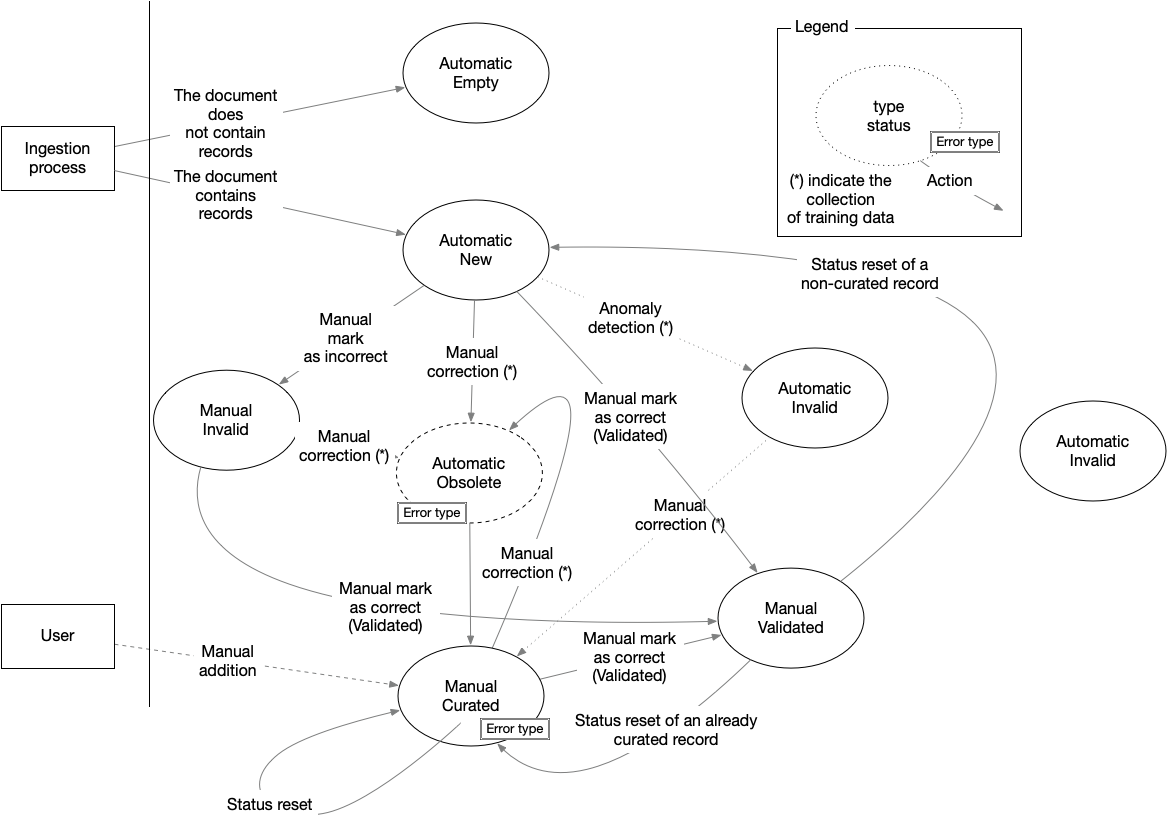
\includegraphics[width=1\textwidth]{images/record-correction} 
  \caption{Schema of the curation workflow. Each state is characterised by two properties: type and status, and one action, as indicated in the top right corner. "Error type" indicates the action of storing the error type for that specific action.}
  \label{fig:curation-workflow}
\end{figure}

\subsubsection{Curation status} 
\label{subsec:curation-status}
The curation status is defined by two internal fields of each record: "status" and "type". 
In Figure~\ref{fig:curation-workflow} they are defined inside each rounded shape. 
The field "status" indicates the record state in the workflow and is summarised in Table~\ref{tab:record-status}.
Some of the "status" values are visible to the users (e.g. validated, curated, invalid) while others (e.g. obsolete, removed) are used internally.
Internal statuses are assigned to records that need to be hidden in the user interface (e.g. removed records are no longer visible).

The status definitions can be summarised as follows: 
\begin{itemize}
    \item \textbf{new}: default status when a new record is created.
    \item \textbf{curated}: the record has been amended manually.
    \item \textbf{validated}: the record was manually marked as valid.
    \item \textbf{invalid}: the record is wrong or inappropriate for the situation (e.g., T\textsubscript{m} or T\textsubscript{curie} extracted as superconducting critical temperature).
    \item \textbf{obsolete}: the record has been updated and the updated values are stored in a new record (internal status).
    \item \textbf{removed}: the record has been removed by a curator (internal status).
\end{itemize}
    
The field "type" indicates whether the record has been modified by a manual or an automatic process. 
For example, the value "automatic" is provided when the data is ingested (Section~\ref{sec:ingestion}) or when the "anomaly detection" detects incorrect values and performs operations such as marking the record "invalid". 
The "type" can change from "automatic" to "manual" but never in the opposite direction, because automatic operations are never applied on validated or curated records.

\subsubsection{Error types}
\label{subsec:error-types}
Error types were first introduced in~\cite{lfoppiano2023automatic} while performing manually the end-to-end evaluation. 
They were combined with the evaluation to provide a more detailed explanation of the reasons why certain extracted values were not correct. 
Since such statistics demonstrated to be useful during the development, we have extended their scope and added additional values related to data curation and validation. 

Selecting the \emph{Error Type} is mandatory in each of the manual actions defined in Figure~\ref{fig:curation-workflow} and it is stored in the "original" record. In the case of an automatic process, anomaly detection sets the \emph{Error Type} with a special status "anomaly detection" to indicate the origin of the modification. 

The error type values can be summarised as follows: 

\begin{itemize}
    \item \textbf{From table}: the entities Material $\rightarrow$ Tc $\rightarrow$ Pressure are identified in a table. At the moment, table extraction is not performed
    \item \textbf{Extraction}: The material, temperature, and pressure are not extracted (no box) or extracted incorrectly. 
    \item \textbf{Linking}: The material is incorrectly linked to the Tc given that the entities are correctly recognised.
    \item \textbf{Tc classification}: The temperature is not correctly classified as "superconductors critical temperature" (e.g., Curie temperature, Magnetic temperature...).
    \item \textbf{Composition resolution}: The exact composition cannot be resolved (e.g., the stoichiometric values cannot be resolved).
    \item \textbf{Value resolution}: The extracted formula contains variables that cannot be resolved, even after having read the paper. This includes when data is from tables
    \item \textbf{Anomaly detection}: The data is automatically modified by the anomaly detection script.
    \item \textbf{Curation amends}: The curator is updating the data which does not present issues due to the automatic system.
\end{itemize}

\subsection{Anomaly detection}
\label{subsec:anomaly-detection}
Anomaly detection is the process of identifying unusual events or patterns in data. 
In our context, this means identifying data that are greatly different from the expected values.
This post-process was introduced in a limited scope to draw attention to certain cases during the curation.

The anomaly detection uses a rule-based approach and marks any record that matches the following conditions:
\begin{itemize}
    \item the extracted T\textsubscript{c} is greater than room temperature (273 K), negative, or contains invalid characters and cannot be parsed (e.g. "41]")
    \item the chemical formula cannot be processed by an ensemble composition parser that combines Pymatgen~\cite{Ong2013}, and text2chem~\cite{kononova_text-mined_2019} 
    \item the extracted applied pressure cannot be parsed or falls outside the range 0 - 250 GPa.
\end{itemize}

Records identified as anomalies are then a) marked as "invalid", and b) attached with a special "error type" called "anomaly detection" for easy identification.
Since this process may find false positives, its output requires validation from curators. 
For example, in certain contexts, T\textsubscript{c} values above room temperature or applied pressure up to 500 GPa may be valid in researchers' hypotheses, calculations, or simulated predictions. 

When we ran the anomaly detection on the full SuperCon\textsuperscript{2} database, it identified 1506 records with invalid T\textsubscript{c}, 5021 records with a chemical formula that was not parseable, and 304 records with invalid applied pressure.  
We also identified only 1440 materials that have been linked to multiple T\textsubscript{c} values. Further analysis and cross-references with this information may be added in future development. 

\subsection{Automatic training data generation}
\label{subsec:feedback-loop-training-data}
The curation process is a valuable endeavour demanding significant knowledge and human effort. 
It is crucial to maximise the use of this time for collecting as much information as possible.
For this reason, we integrated an automatic procedure in the curation process for accumulating examples that can be used for training data in ML models. 

Since the training data generated are related to manual corrections, they are targeting real mistakes from the ML model. 
In Section~\ref{subsec:training-data-generation-evaluation} we demonstrate they have a relevant impact on improving the ML model with a small number of examples as compared with the training dataset. 

\subsubsection{Training data collection}
In the event of a change (update, removal) in a database record, this process retrieves the corresponding raw data: the text passage, the recognised entities (spans), and the layout tokens information. 
This information is sufficient to be exported as training examples, which can be examined and corrected, and feedback to the ML model. 

In detail, the process performs the following actions:
\begin{itemize}
    \item The updated record is prepared and stored.
    \item The raw data originating the updated record is identified. First, the corresponding structured document is retrieved from the document collection using the document identifier (the hash). Then, the exact text passage in the structured document is located using a unique id assigned to each material in the database records.
    \item If the raw data has already been collected, it is skipped. This is the case when multiple records belonging to the same text passage are corrected.
    \item Otherwise, the raw information comprising the text string, the spans, and the layout tokens are collected and saved in a separate collection.
    \item The data collected is then sufficient to generate workable instances in different output formats and the related feature files.
\end{itemize}

\subsubsection{Training data management}
We designed a specific page of the interface (Section~\ref{sec:user-interface}) to manage the collected data (Figure~\ref{fig:training-data-view}) in which each row corresponds to a training example, which includes the decorated text showing the identified entities, the document identifier, and the status. 
The users can examine the data, delete it, or send it to the annotation tool to be corrected. 
Depending on which state the records are in, the status can be: "new" when the data is added, "in progress" after the data is sent to the annotation tool, and "exported" when the corrected training data is downloaded. 
We integrated Label-studio~\cite{Label_Studio} for the correction of the collected. Label-studio is an open-source, python-based, and modern interface supporting many different TDM tasks (NER, topic modelling, image recognition, etc.). 

\begin{figure}[ht]
  \centering
  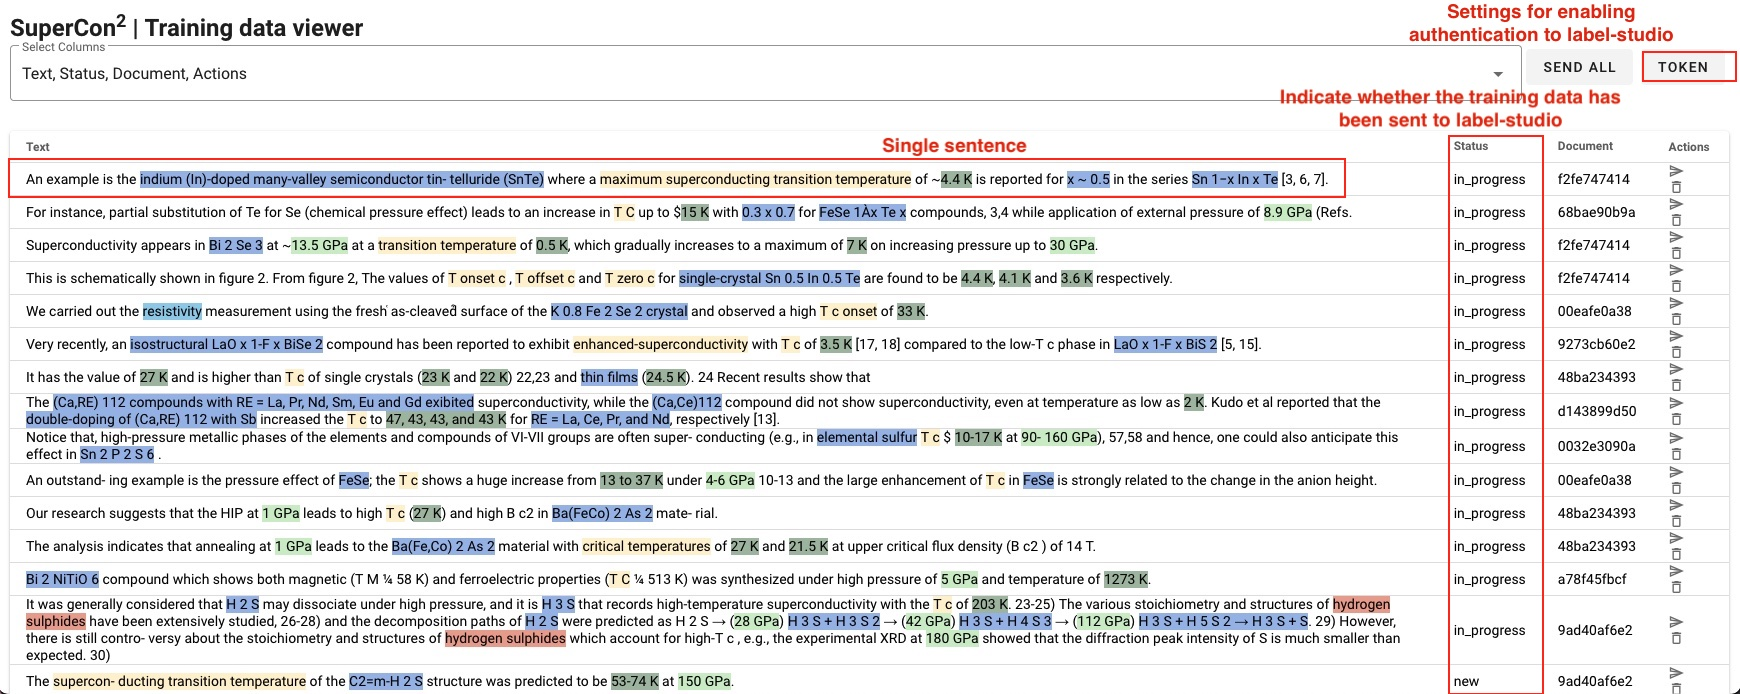
\includegraphics[width=1\textwidth]{images/training-data-viewer} 
  \caption{Training data view}
  \label{fig:training-data-view}
\end{figure}

\section{Curation interface}
\label{sec:user-interface}

The workflow is operated through the user interface, which offers several key features to facilitate the data curation process.
It provides a comprehensive view of materials and their related properties as a table which includes search, filtering, and sorting functionality (Figure~\ref{fig:curation-interface-database}). 
The schema consists of two main classes: material information (material names, formulas, shape, etc.), properties (T\textsubscript{c}), and conditions (applied pressure, measurement method, etc.). The complete list including examples is reported in our previous work~\cite{lfoppiano2023automatic}.

\begin{figure}[ht]
  \centering
  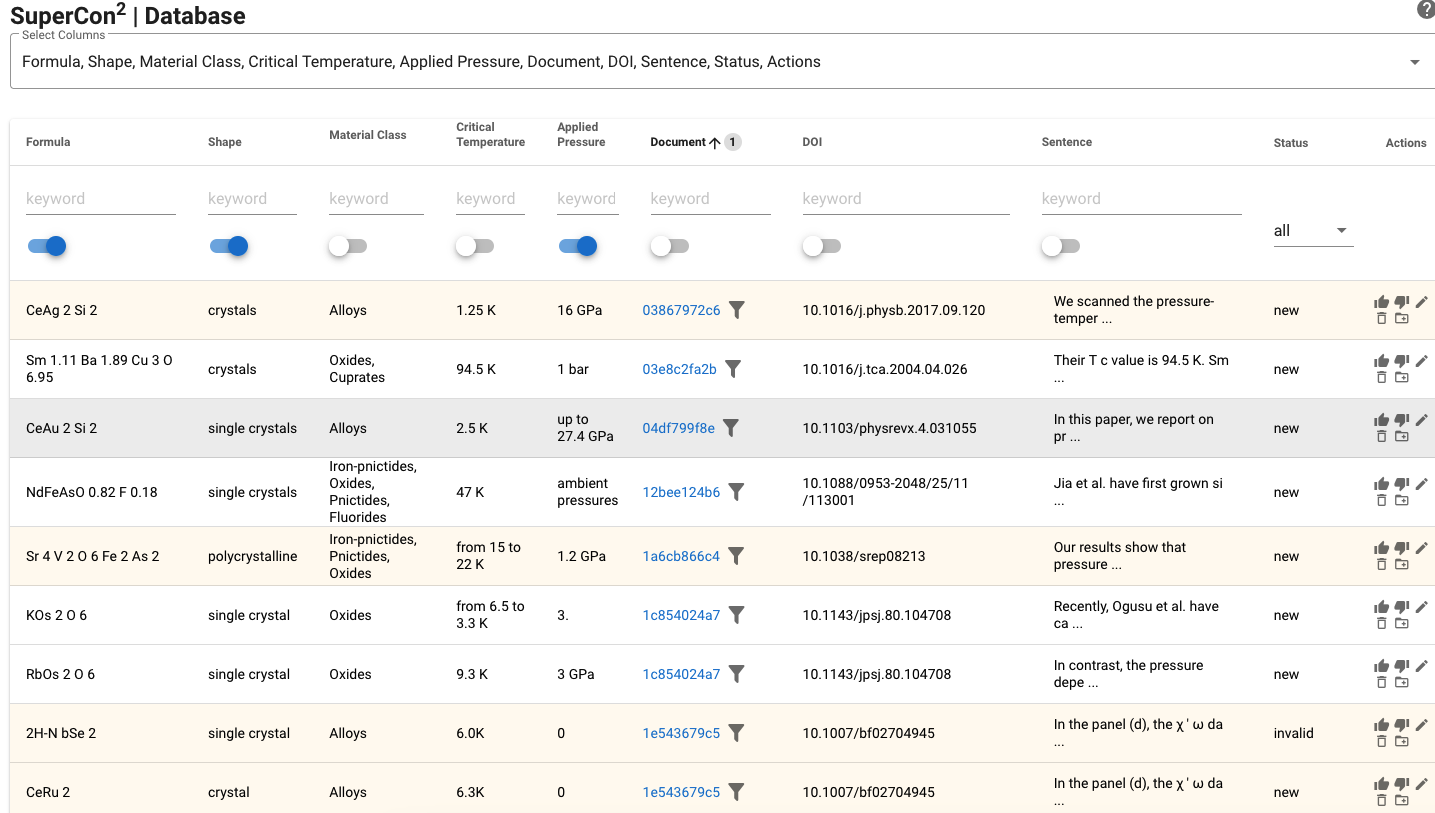
\includegraphics[width=1\textwidth]{images/supercon-curation-database} 
  \caption{Curation interface showing the database as a table}
  \label{fig:curation-interface-database}
\end{figure}


During the curation process, it is often necessary to switch back and forth between the database record and the related context in the paper (the related paragraph or sentence). 
Our interface provides a viewer for individual documents, which visualises in the same window a table with the extracted records and the original PDF document (Figure~\ref{fig:pdf-view}). 
The PDF document is decorated with annotations that identify the extracted materials and properties, enabling users to easily locate and reference the extracted information within the document.

Through the interface, users can add, amend, remove, or mark each of the records in the database.
Marking a record imply declaring explicitly the record as invalid or valid.
Adding new records is limited to documents already in the database. 
When a record is added to a document, the record's bibliographic data are copied from other records in the same documents and the user has to only care filling up the correct experimental information (material, Tc, etc.).


% The interface automatically collects training data; when a record is amended, the information pertaining it's raw source information (sentence text, annotations) are collected (Section~\ref{subsec:feedback-loop-training-data}). 

\begin{figure}[ht]
  \centering
  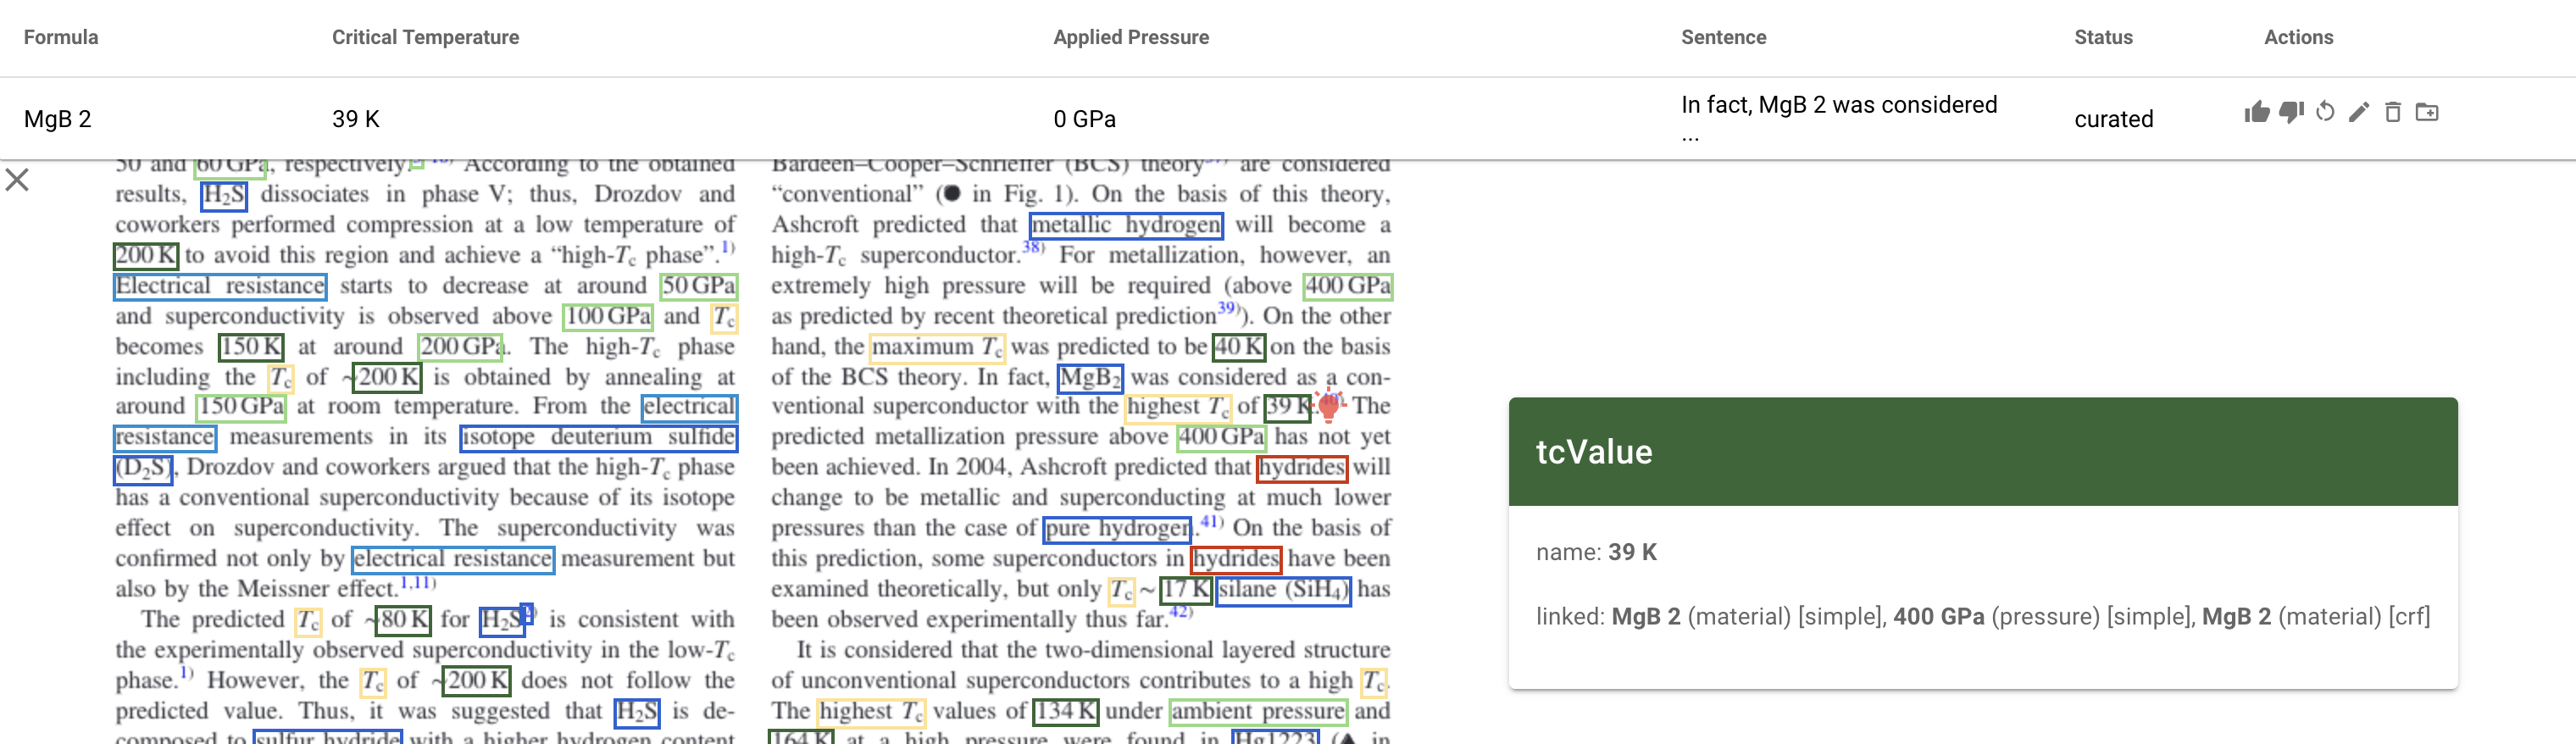
\includegraphics[width=1\textwidth]{images/pdf-view-context.png} 
  \caption{PDF document viewer showing an annotated document. The table on top is linked through the annotated entities. The user can navigate from the record to the exact point in the PDF, with a pointer (the red bulb light) identifying the context of the entities being examined. }
  \label{fig:pdf-view}
\end{figure}

% \begin{figure}[ht]
%   \centering
%   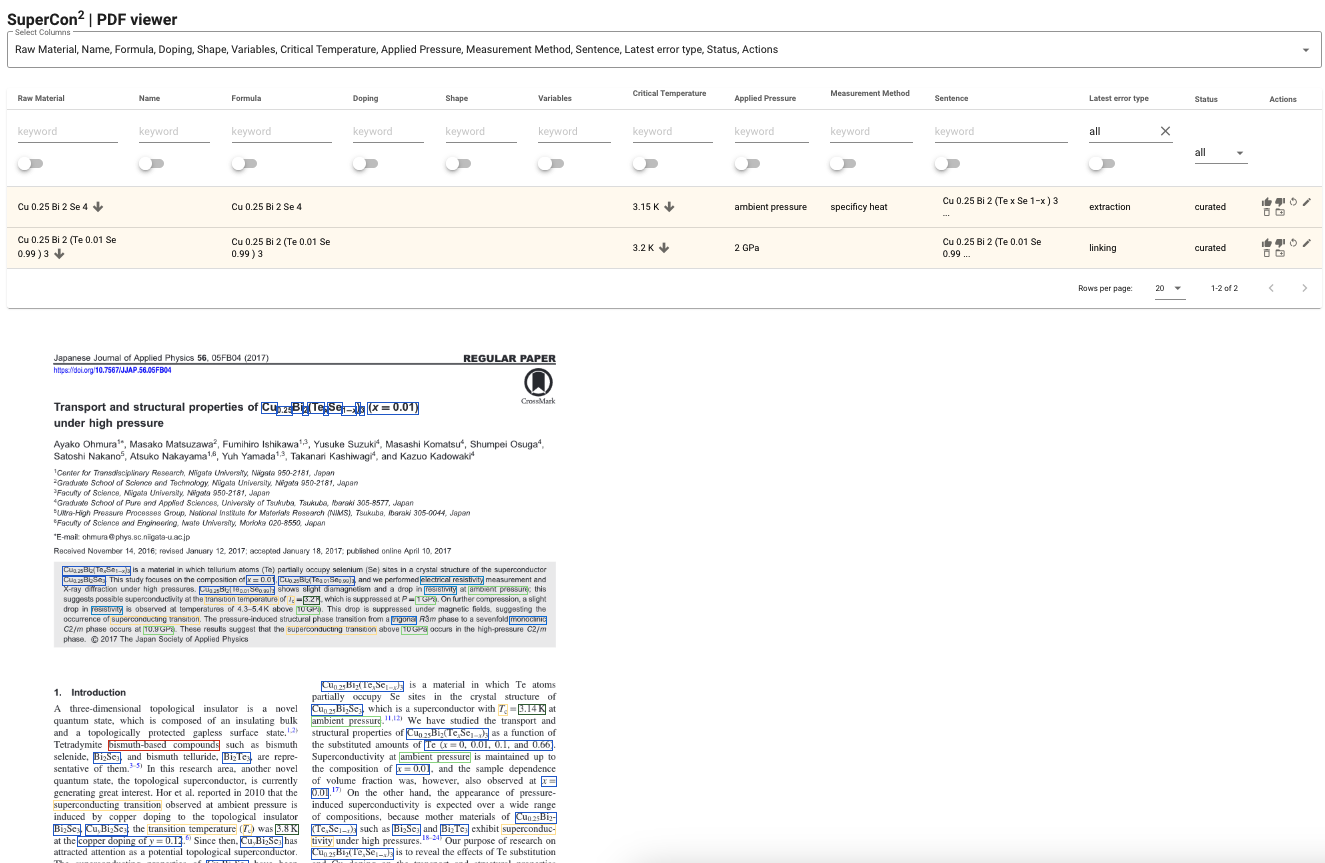
\includegraphics[width=1\textwidth]{images/supercon-curation-pdf-viewer} 
%   \caption{PDF viewer. The page includes a table showcasing records extracted from the  current document, along with the PDF content and accompanying annotations.}
%   \label{fig:curation-interface-pdf-viewer}
% \end{figure}


\subsection{Manual curation approach}
\label{sec:data-correction}
\label{subsec:manual_correction}

Manual curation is still indispensable for developing high-quality structured data since the data extracted automatically may contain incorrect information.
We have set up an automatic process for anomaly detection (Section~\ref{subsec:anomaly-detection}) which can help to speed up the process but it only detects "potential" problems and requires anyway a manual validation.

To certify the gold-standard data quality, we employ only curators from domain experts in the field. 
Although, even among experts, experience plays an important role (Section~\ref{sec:interface-evaluation})
To avoid worker dependence and ensure robustness in the process, we took two approaches. 
First, we used a double-round approach where the data is initially corrected by one person, and validated in a second round, by a different person. 
Second, we have built documentation for the curation as a form of guidelines through an iterative loop of processes, as discussed in our previous work on the construction of the annotated dataset SuperMat~\cite{foppiano2021supermat}. 

The loop includes four steps: 
\begin{itemize}
    \item collect rules, based on observation and reasoning,
    \item curation following those rules,
    \item retrospective including analysis and discussions based on curators' feedback, and
    \item take decisions and update the guideline
\end{itemize}

\subsection{Curation guidelines}

The guidelines consist mainly of two parts: the general principles and the correction rules with examples of solutions.
The guidelines are designed to provide general information applied to corrections and very basic explanations containing illustrations for a faster understanding (e.g. the meaning of the colours of the annotations). This would help new curators to catch up with the required level of curation precision quickly. 
There are two main components described in the correction rules: the record that is being corrected and its context. 
The context of a record can be obtained by examining the extracted annotated text or the PDF document area.

The correction rules are described based on the error type mentioned in Section~\ref{subsec:error-types}, and in the guideline, the description of rules is accompanied by sheets that explain five points to the curators, as illustrated in Figure~\ref{fig:example-curation-sheet}:
\begin{itemize}
    \item \textbf{Sample input data}, a screenshot of SuperCon\textsuperscript{2} record in the interface
    \item \textbf{Context}, a screenshot of the related part of the document (either from the PDF or from plain text sentences) that contain the extracted data to be curated,
    \item \textbf{Motivation}, describes the issue with the examined extracted data, 
    \item \textbf{Action} to be taken, 
    \item \textbf{Expected output}, a screenshot of the expected SuperCon\textsuperscript{2} record, after correction
\end{itemize}

% An example of a sheet can be found in Figure~\ref{fig:example-curation-sheet}. 

\begin{figure}[ht]
  \centering
  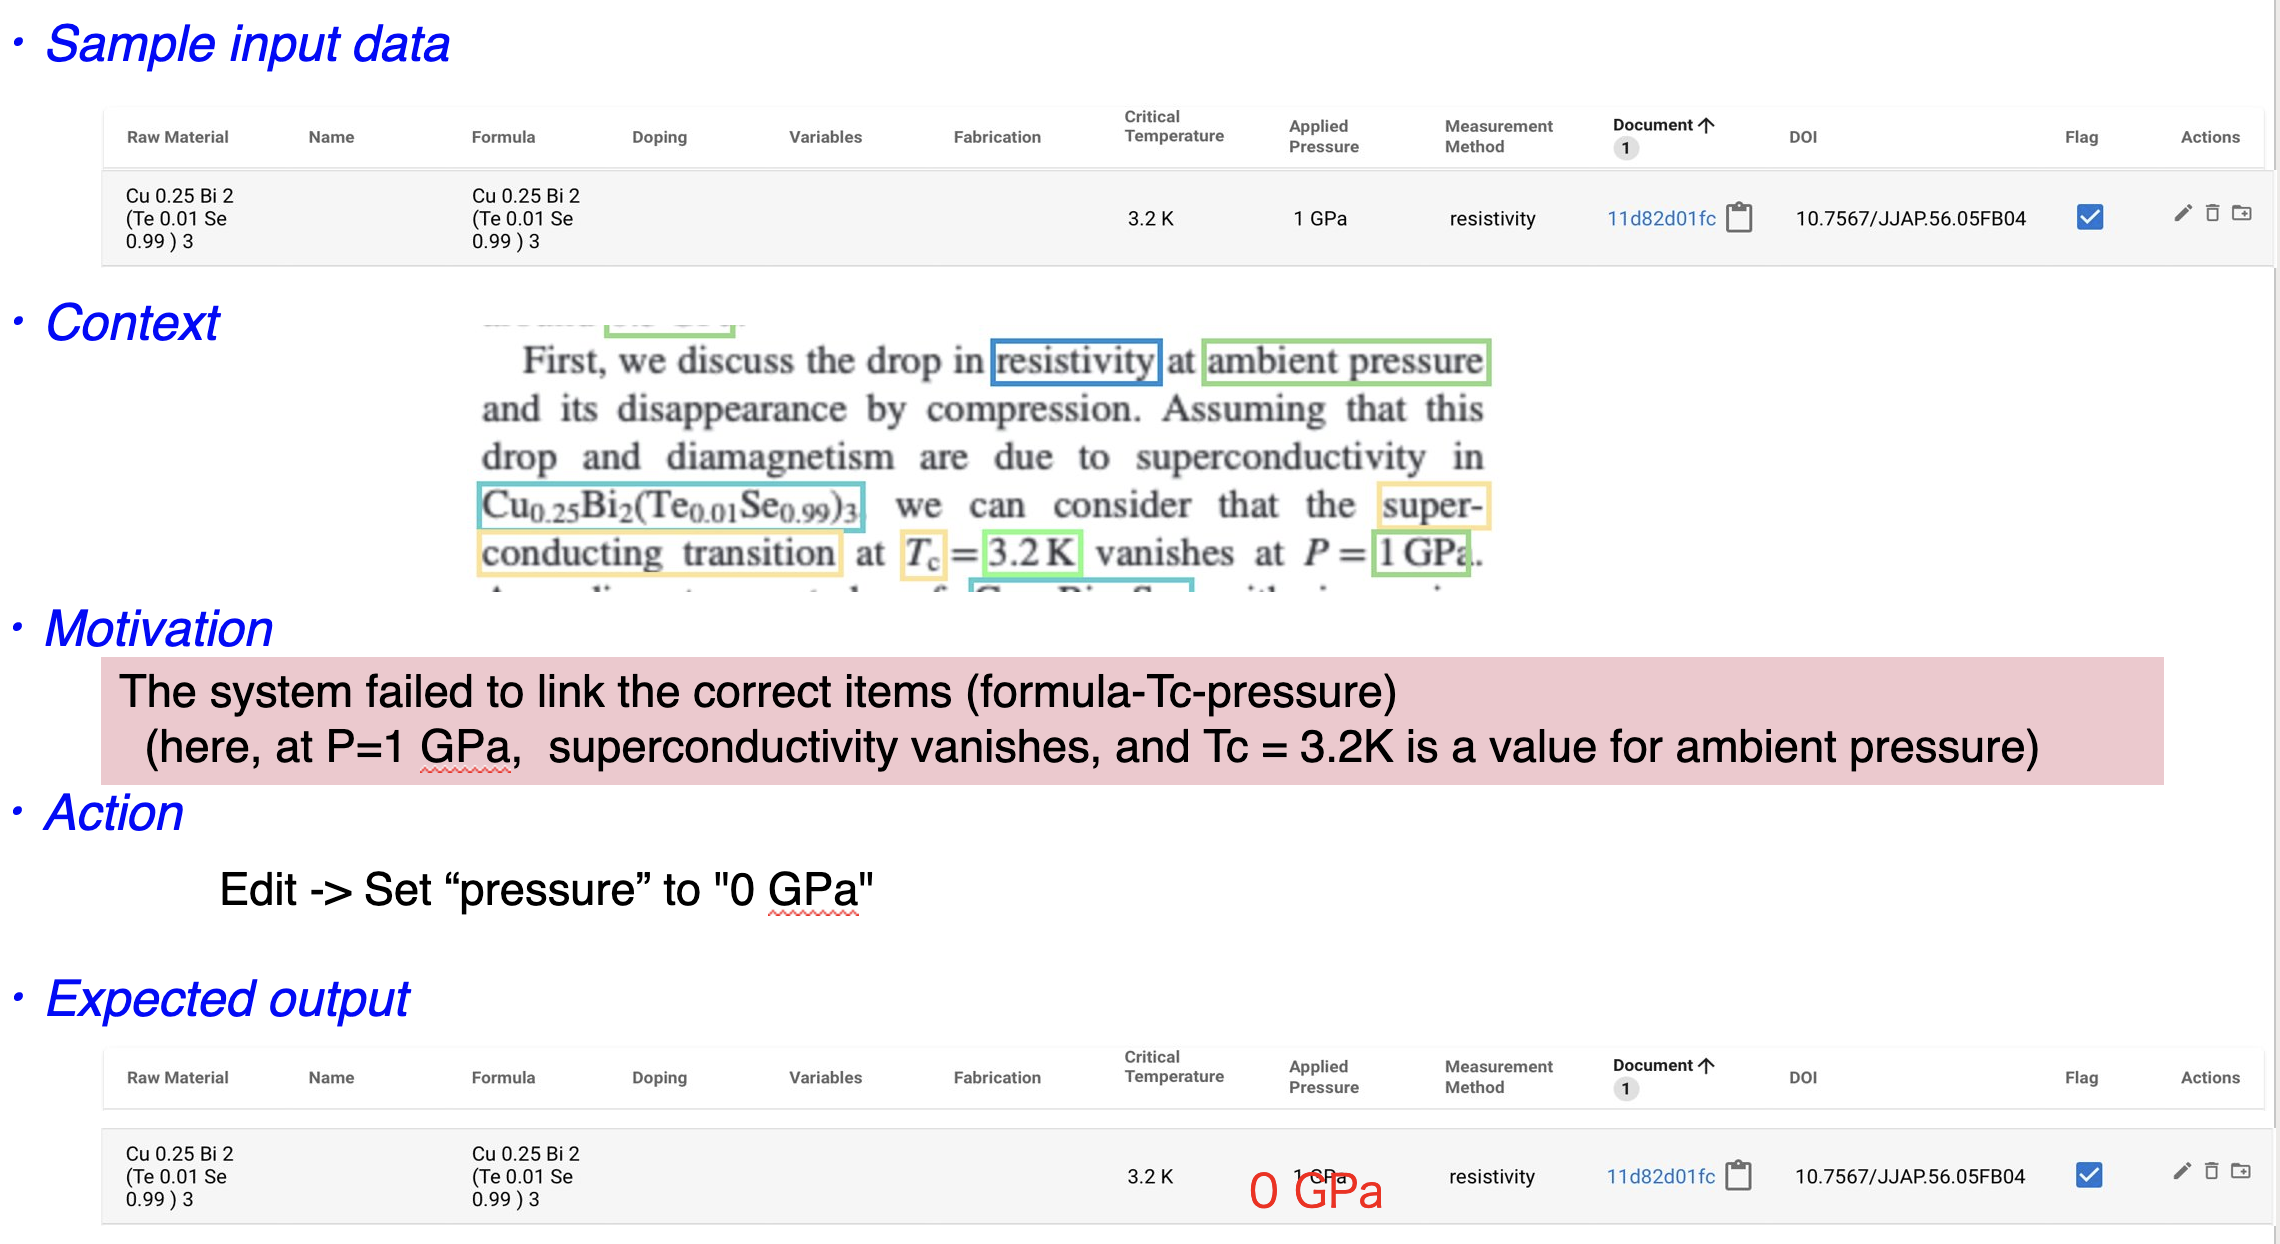
\includegraphics[width=1\textwidth]{images/example-sheet-curation.png} 
  \caption{Example of curation sheet. As discussed, it's written with simple language assuming the curator may not be familiar with the task. }
  \label{fig:example-curation-sheet}
\end{figure}


\subsection{Curation and processing logs}
\label{subsec:curation-and-processing-logs}

The Supercon\textsuperscript{2} interface gives access to information regarding the ingestion (processing log) and the curation process (curation log). 
The processing log is filled up when the data is ingested, it was built to have minimal functions able to explain why certain documents haven't been processed (Figure~\ref{fig:processing-curation-log}). 
For example, sometimes documents are failing because they don't contain any text (image PDF documents) or they are too big (more than 100 pages). 
% Grobid was built focusing on speed and robustness, and contains several fail-safe mechanisms to avoid crashing the system when a document is either too big or does not contains valuable information, for example, does not have any text. 
% Old PDF documents (e.g. before 1990) are likely to have been scanned and contain only images. 
% Examples of too big documents are dissertation theses with more than 100 pages, that might be collected by mistake. 


\begin{figure}[ht]
  \centering
  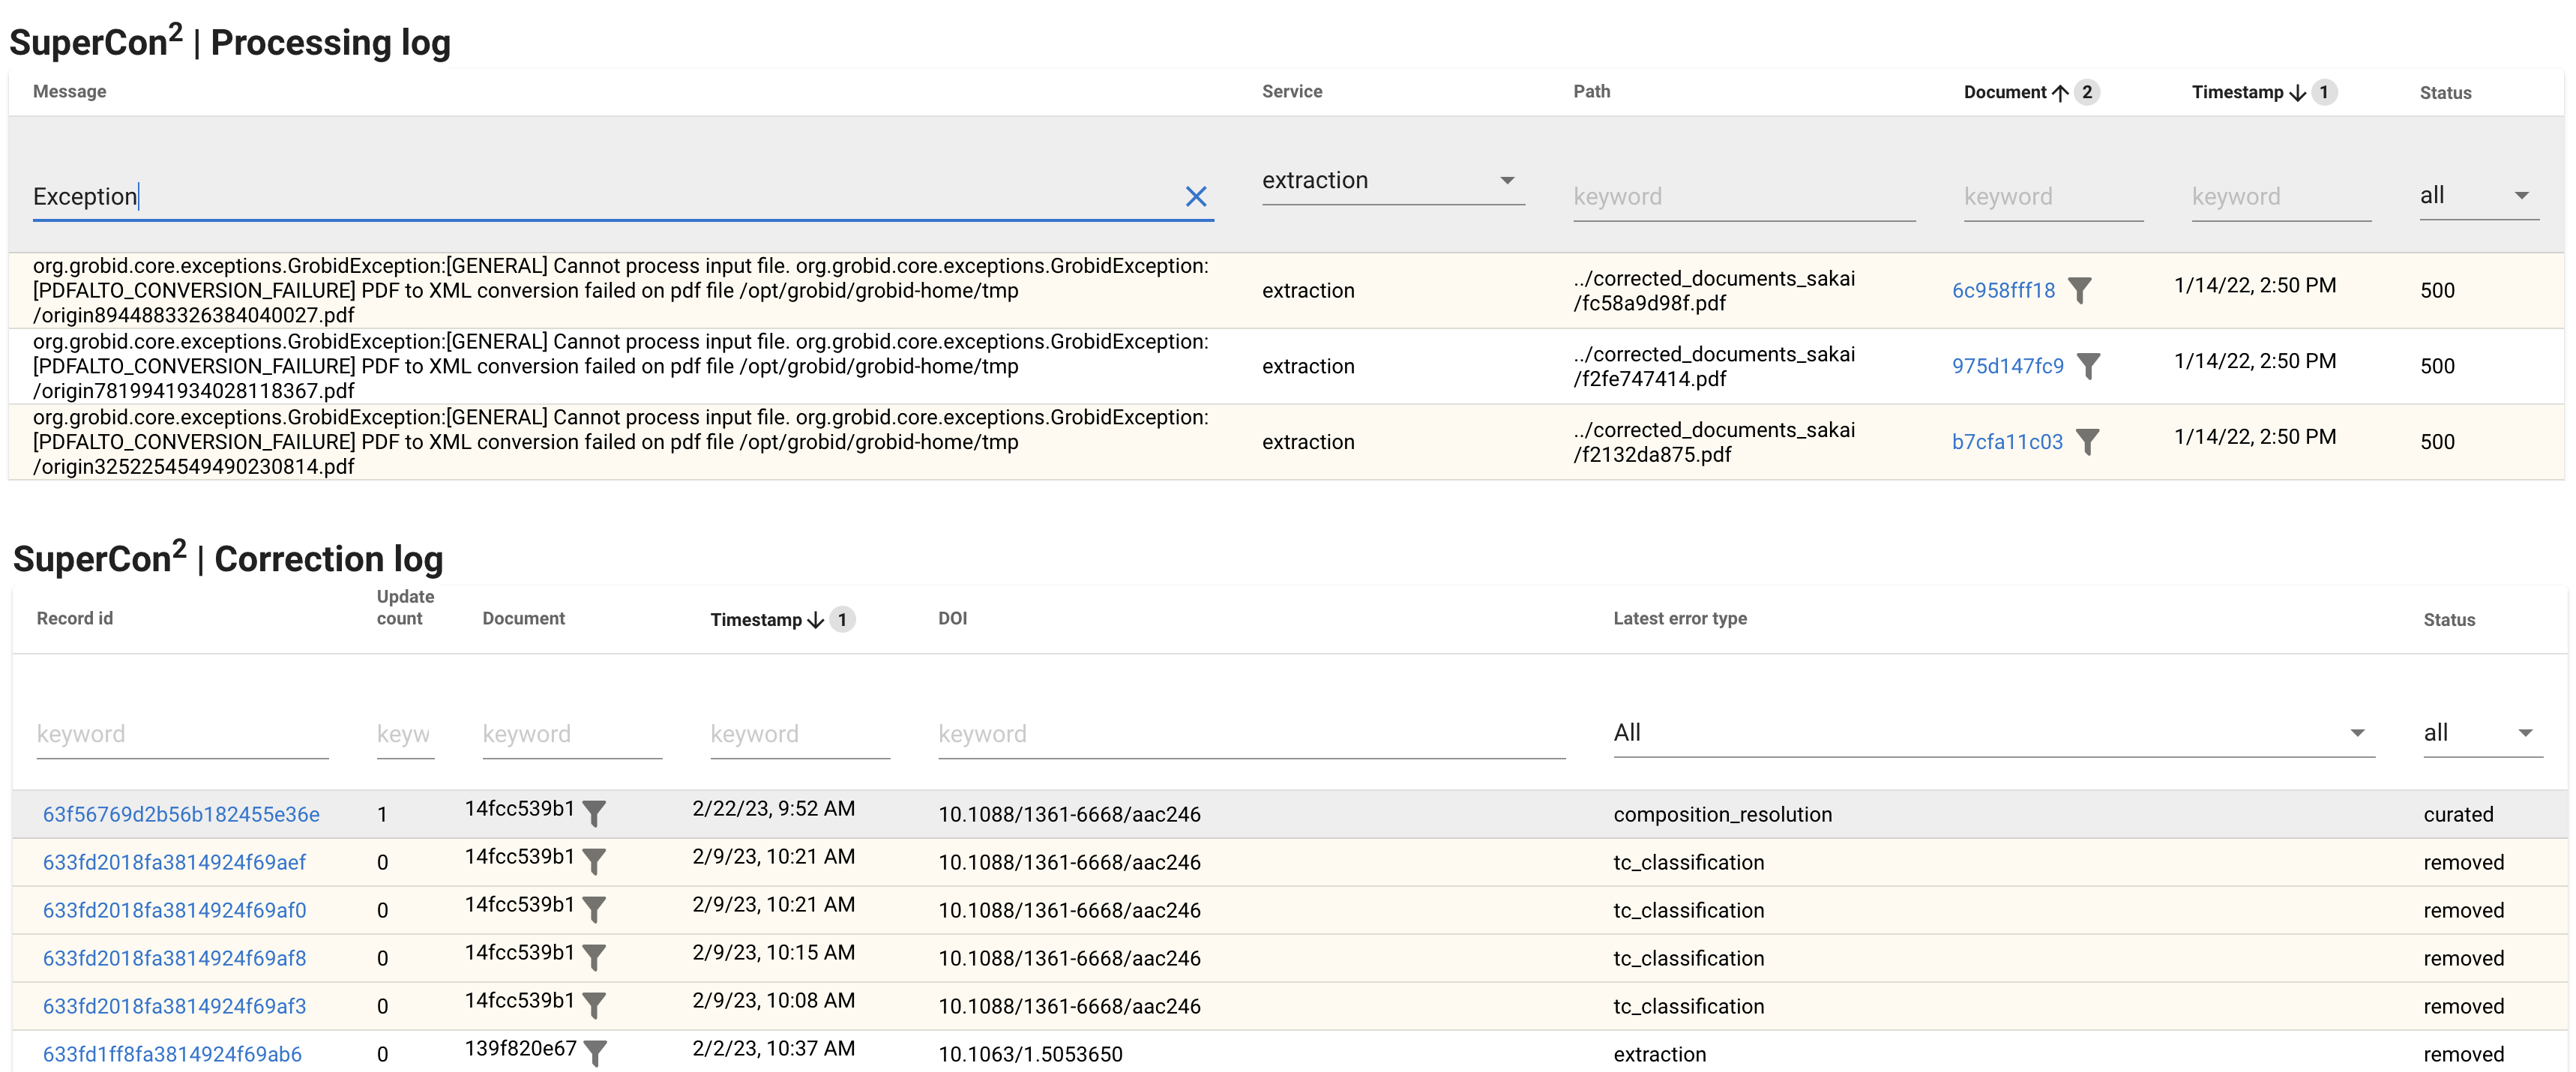
\includegraphics[width=1\textwidth]{images/processing-curation-log.png} 
  \caption{On the top: Processing log, showing the output of each operation (process document, create a record) and the outcome with the exception or error that should have occurred. On the bottom: Curation log, indicating each record, the number of updates, and the date/time of the last updates.}
  \label{fig:processing-curation-log}
\end{figure}

The curation log provides a view of what, when and how a record has been corrected (Figure~\ref{fig:processing-curation-log}).

% \begin{figure}[ht]
%   \centering
%   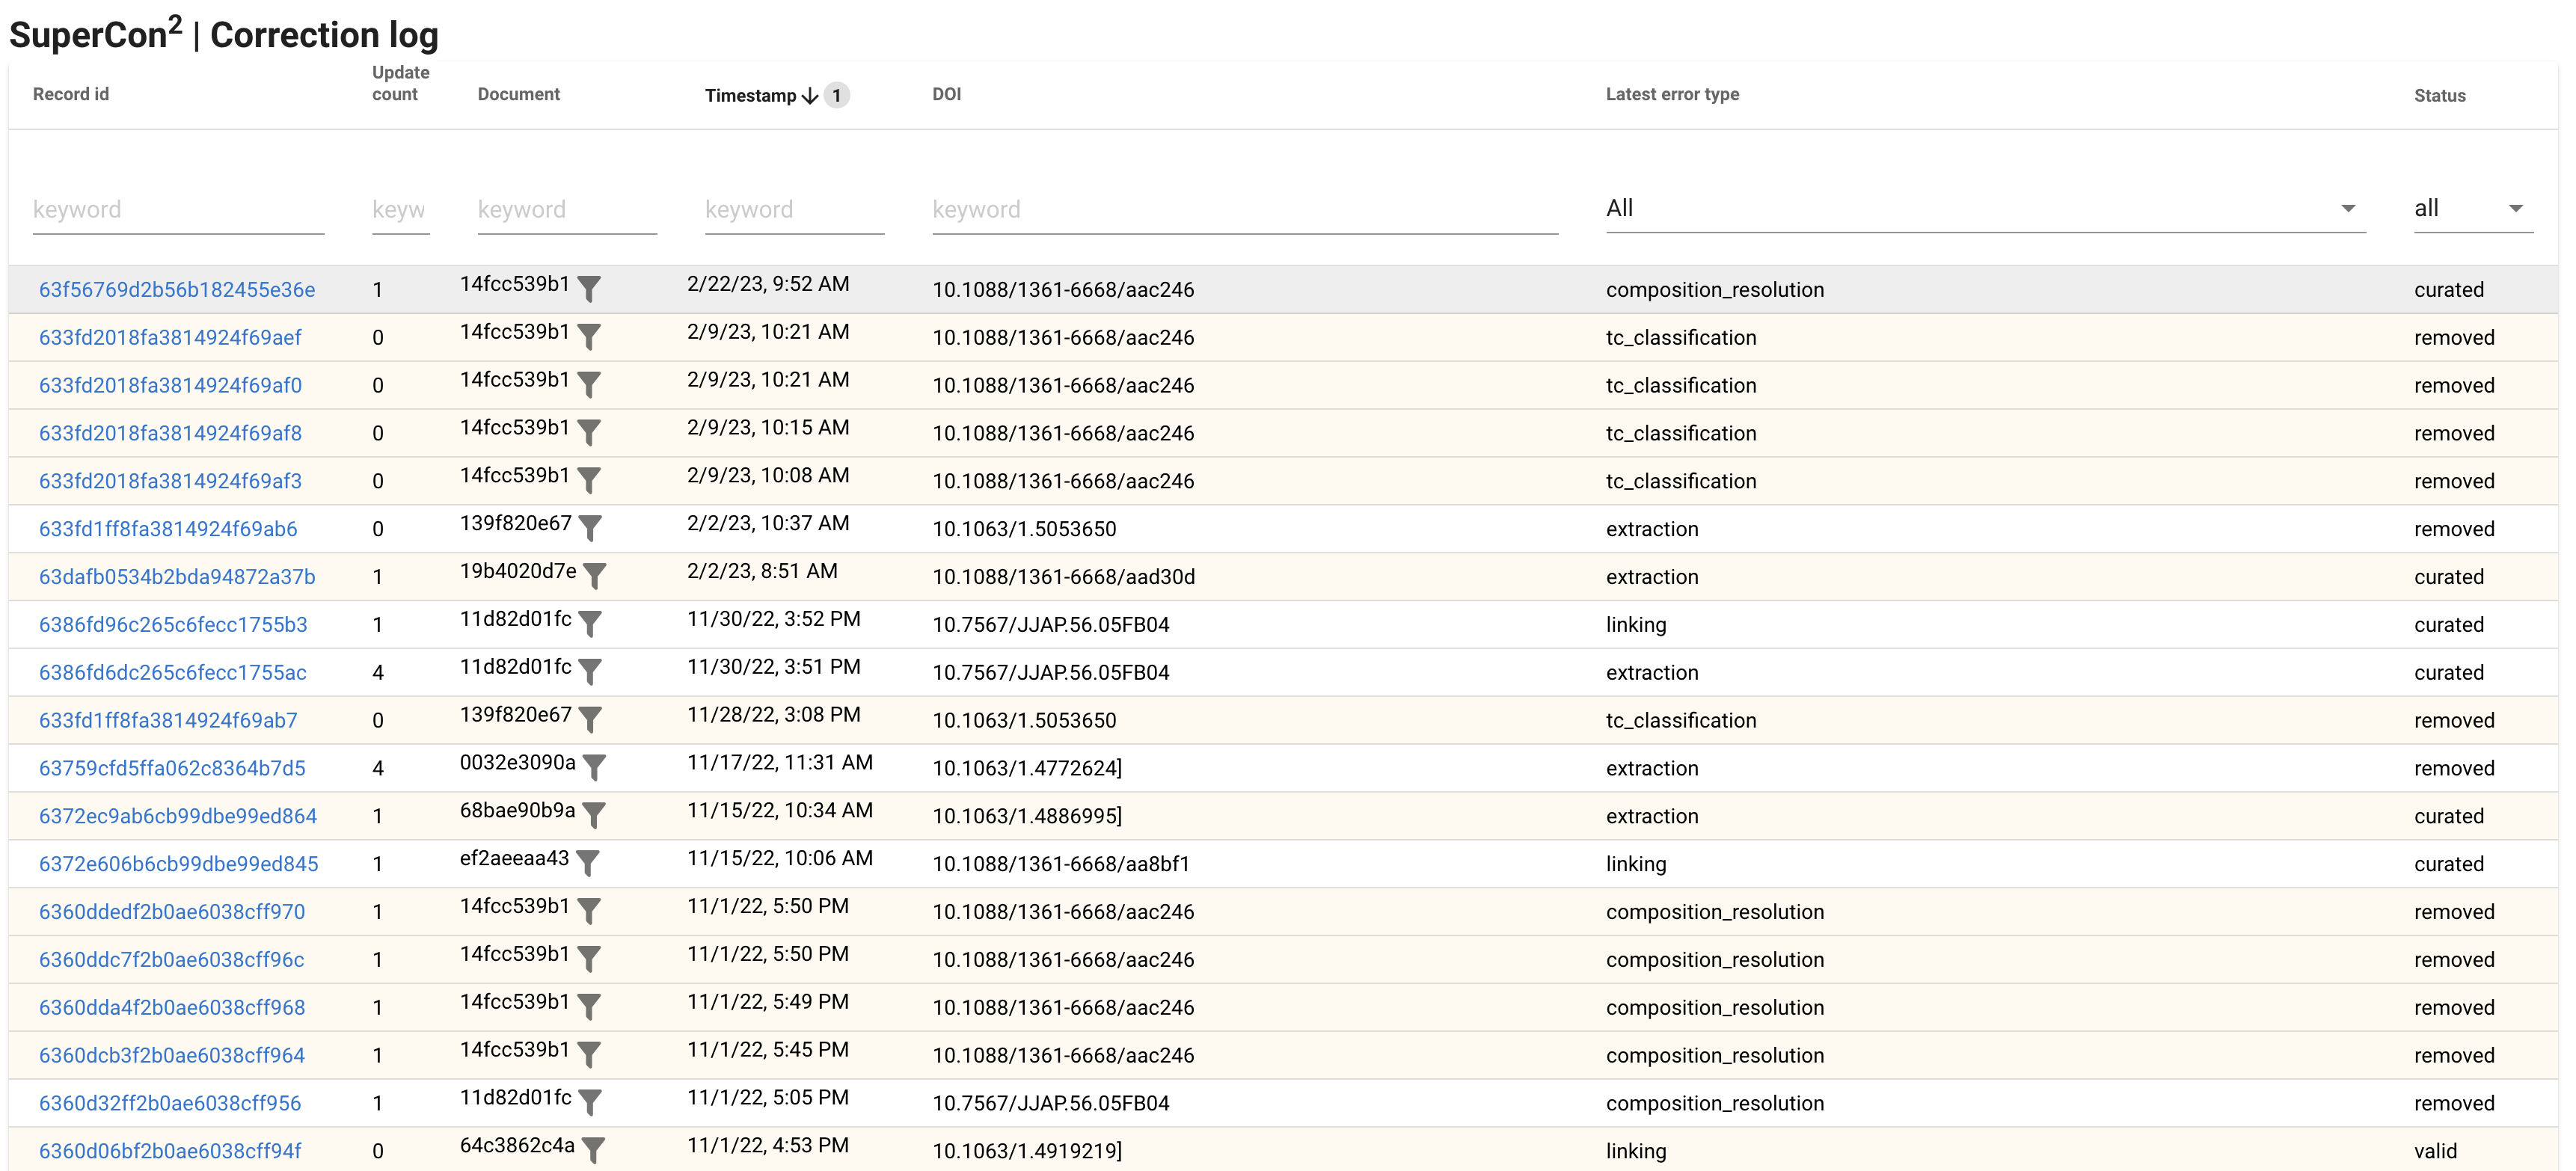
\includegraphics[width=1\textwidth]{images/curation-log} 
%   \caption{Curation log, indicating each record, the number of updates, and the date/time of the last updates. }
%   \label{fig:curation-log}
% \end{figure}




\section{Results and evaluation}

In this section, we illustrate the experiments we have run to evaluate our work. 
The evaluation is composed of three sets of results. 
The anomaly detection rejection rate (Section~\ref{subsec:anomaly-detection-evaluation}) indicates how many anomalies were rejected by curators after validation. 
Then, we demonstrate that the training data automatically selected contributed to improving the ML model with a small set of examples (Section~\ref{subsec:training-data-generation-evaluation}) 
Finally, we evaluated the quality of the data extraction using the interface (and the semi-automatic TDM process) against the classical method of reading the PDF articles and noting the experimental information in an Excel file. In Section~\ref{sec:interface-evaluation} we find that using the interface improves the quality of the curated data and in particular in terms of recall, where the interface helps reduce the missing experimental data. 


\subsection{Anomaly detection rejection rate}
\label{subsec:anomaly-detection-evaluation}

We evaluate the anomaly detection and examined the detected anomalies rejected by human validation. 
We considered a small subset of the database containing 667 records. 
The detection found 17 anomalies in T\textsubscript{c}, 1 anomaly in applied pressure, and 16 anomalies in the chemical formulas. 
The percentage of anomaly detection results rejected by curators after rechecking was 23\% for Tc, 37\% in chemical formulas and 0\% for applied pressure. 
This indicates appropriate effectiveness and a relatively low rate of false positives, although a detailed study might be needed due to the small sample size.

\subsection{Training data generation}
\label{subsec:training-data-generation-evaluation}
We selected around 400 Supercon\textsuperscript{2} extracted records initially marked by the anomaly detection process. 
Following the guidelines, we corrected these records to exclude false positives wrongly identified by anomaly detection.  
At the same time the interface collected examples of training data based on our corrections. 
Then, after we corrected the obtained set of raw data we obtained a small set of 352 training data examples for our superconductors ML models. 
We call the obtained dataset \emph{curation} to be distinguished from the original SuperMat dataset which is referred to as \emph{base}.

We prepared our experiment using the SciBERT~\cite{Beltagy2019SciBERT} implementation, and we fine-tuned the model for our downstream NER task discussed in detail in~\cite{lfoppiano2023automatic}.
We trained five models, and evaluate them using a fixed holdout dataset from SuperMat, and we averaged the results for smoothing out the fluctuations in the results. 
We use the DeLFT (Deep Learning For Text)~\cite{DeLFT} library for training, evaluating, and managing the models for prediction.  
A model can be trained with two different strategies: 
\begin{enumerate}
    \item \emph{``from scratch''}: when the model is initialised randomly. We denote this strategy with an \emph{(s)}.
    \item \emph{``incremental''}: when the initial model weights are taken from an already existing model. We denote this strategy with an \emph{(i)}.
\end{enumerate}
The latter can be seen as a way to ``continue'' the training from a specific checkpoint.

We thus define three different training protocols: 
\begin{enumerate}
    \item \textbf{base(s)}: using the \emph{base} dataset and training from scratch (s).
    \item \textbf{(base+curation)(s)}: using both the \emph{base} and \emph{curation} datasets and training from scratch (s).
    \item \textbf{base(s)+(base+curation)(i)}: Using the \emph{base} dataset to train from scratch (s), and then continuing the training with the \emph{curation} dataset (i).
\end{enumerate}
We merge ``curation'' with the base dataset because the curation dataset is very small compared to ``base'', and we want to avoid catastrophic forgetting~\cite{overcoming-kirkpatrick-etal-2016} or overfitting.

The trained models are then tested using a fixed holdout dataset that we designed in our previous work~\cite{lfoppiano2023automatic} and the evaluation scores are shown in Table~\ref{tab:evaluation-curation-training2}.

\begin{table}[ht]
\centering\small
\caption{F1-score from the evaluation of the fine-tuning training of SciBERT. The training is performed with three different approaches. 
The \emph{base} dataset is the original dataset described in~\cite{lfoppiano2023automatic}, and the \emph{curation} dataset is automatically collected based on the database corrections by the interface and manually corrected. \textit{s} indicate "training from scratch", while \textit{i} indicate "incremental training". 
The evaluation is performed using the same holdout dataset from SuperMat. 
The results are averaged over 5 runs. }
\begin{tabular}{lrrr}
\toprule
& \textbf{base(s)} & \textbf{(base+curation)(s)} & \textbf{base(s)+curation(i)} \\ 
\midrule
Nb total examples & 16902 & 17254 & 16902(s), 17254 (i)\\ 
\midrule
\texttt{<class>}        & 70.41         & \textbf{73.02}         & 71.86 \\ 
\texttt{<material>}     & 79.37         & 80.09         & \textbf{80.37} \\ 
\texttt{<me\_method>}   & 66.72         & 66.57         & \textbf{66.95} \\ 
\texttt{<pressure>}     & 46.43         & \textbf{48.42}         & 47.23 \\ 
\texttt{<tc>}           & 80.13         & \textbf{80.92}         & 80.34 \\ 
\texttt{<tcValue>}      & 78.29         & 78.41         & \textbf{79.73} \\ 
\midrule
\textbf{All (micro avg.)} & 76.67       & 77.44         & \textbf{77.48} \\ 
\midrule
\textbf{$\Delta$ avg. w/ baseline}& -   & +0.77     & \textbf{+0.81} \\ 
\bottomrule
\end{tabular}
\label{tab:evaluation-curation-training2}
\end{table}


\begin{table}[ht]
\centering
\caption{Data support: number of entities of a specific type in the training dataset.}
\begin{tabular}{lrrr}
\toprule
                        & \textbf{base}     & \textbf{base+curation}    & \textbf{$\Delta$}  \\ 
\midrule
\texttt{<class>}        & 1646              & 1732                      &  86                \\
\texttt{<material>}     & 6943              & 7580                      &  637               \\
\texttt{<me\_method>}   & 1883              & 1934                      &  51                \\
\texttt{<pressure>}     & 274               & 361                       &  87                \\
\texttt{<tc>}           & 3741              & 4269                      &  528               \\
\texttt{<tcValue>}      & 1099              & 1556                      &  457               \\
\midrule
\textbf{Total}          & 15586             & 17432                     & 1846               \\ 
\bottomrule
\end{tabular}
\label{tab:training-support}
\end{table}


This experiment demonstrates that with only 352 examples (2\% of the SuperMat dataset) comprising 1846 additional entities (11\% of the entities from the SuperMat dataset) (Table~\ref{tab:training-support}), we obtain an improvement from 76.67\%\footnote{In our previous work~\cite{lfoppiano2023automatic} we reported 77.03\% F1-score. 
There is slight a decrease in absolute scores between DeLFT 0.2.8 and DeLFT 0.3.0. 
One cause may be the use of different hyperparameters in version 0.3.0 such as batch size and learning rate.
However, the most probable cause could be the impact of using the Huggingface library which is suffering from quality issues in relation to their tokenizers implementation \url{https://github.com/kermitt2/delft/issues/150}.} to an F1-score between 77.44\% (+0.77) and 77.48\% (+0.81) for (base+curation)(s) and (base(s)+curation(i)), respectively. 

% Here, the incremental approach obtained a score similar to the model trained from scratch with the extended ``base+curation'' dataset. 
% There are several hypotheses for this result, the first hypothesis is that the training dataset is not big enough for the task at hand, therefore the model requires more training time. 
% This issue could be verified by correcting all the available training data and repeating this experiment. 
% Another hypothesis that our data distribution is rather skewed (c.f. Table \ref{tab:training-support}) favours an incremental approach as the deltas in the support of the ``curation'' dataset with respect to the ``base'' dataset, somehow counters the class imbalance. 

This experiment gives interesting insight relative to the positive impact on the way we select the training data. 
However, there are some limitations: the \emph{curation} dataset is small as compared with the \emph{base} dataset. This issue could be verified by correcting all the available training data and repeating this experiment, and studying the interpolation between the size of the two datasets and the obtained evaluation scores. 
A second limitation is that the hyperparameters we chose for our model, in particular, the learning rate and batch size could be still better tuned to obtain better results with the second and third training protocols.


\subsection{Data quality}
\label{sec:interface-evaluation}
We conducted an experiment to evaluate the effectiveness and accuracy of data curation using two techniques: a) the user interface, and b) the traditional manual method involving reading PDF documents and populating an Excel file.

We opted for a sample dataset consisting of 15 papers, which we divided among three curators — a senior researcher, a PhD student, and a master's student. Each curator received 10 papers, with an equal distribution between using the \textit{interface} and working with \textit{pdf} files. 
There was an overlap of 5 papers between curators, where the opposite method was applied. 
For instance, if curator A used the \textit{interface} to correct paper 1, curator B, who also had the same paper, corrected it by reading the \textit{pdf} document.
After curation, a fourth individual manually reviewed the curated content. The revisions made during this process were then employed to calculate the evaluation scores.

We assessed the two approaches using a dual perspective: efficiency, by contrasting the time needed for curation, and accuracy, quantified through precision, recall, and the F1-score.

\subsubsection{Discussion}
The comparison of the time taken revealed no significant difference between the interface and the traditional method. Specifically, the total time was only 4 minutes longer with the interface (188 minutes compared to 184 minutes). The time difference did not demonstrate any consistent trend, suggesting the need for a larger dataset in future experiments.

When we examined the accuracy of the extracted data, we observed a 6\% improvement in precision and a substantial 111\% improvement in recall when using the interface (Table~\ref{tab:evaluation-interface-correction}). 

\begin{table}[ht]
\centering\small
\caption{Evaluation scores (P: precision, R: recall, F1: F1-score) between the curation using the SuperCon 2 interface (Interface) and the traditional method of reading the PDF document (PDF document). }
\begin{tabular}{lrrr}
\toprule
                    & \textbf{P (\%)}   & \textbf{R (\%)}   & \textbf{F1 (\%)}  \\
    \midrule
    PDF document    & 87.83             & 45.60             & 52.66             \\
    Interface       & \textbf{93.37}    & \textbf{96.39}    & \textbf{93.28}    \\
    \bottomrule
\end{tabular}
\label{tab:evaluation-interface-correction}
\end{table}

The disparity in experience significantly influenced the accuracy of curation, particularly in terms of high-level skills. Senior researchers consistently achieved an average F1-Score approximately 20\% higher than other curators (see Table~\ref{tab:accuracy-by-experience}). Furthermore, we observed a modest improvement between master's students and PhD students. These findings indicate also that for large-scale projects, employing master students instead of PhD students may be a more cost-effective choice. Thus, using only a few senior researchers for the second round of validation (Section~\ref{subsec:manual_correction}).

\begin{table}[h]
\centering
\caption{Evaluation scores (P: precision, R: recall, F1: F1-score) aggregated by experience}
\begin{tabular}{lrrr}
\toprule
\textbf{Experience} & \textbf{P (\%)}   & \textbf{R (\%)}   & \textbf{F1 (\%)}  \\
\midrule
Master student      & 90.03             & 66.10             & 66.40             \\
PhD student         & 83.33             & 65.69             & 69.45             \\
Senior researcher   & \textbf{98.45}    & \textbf{81.22}    & \textbf{83.08}    \\
\bottomrule
\end{tabular}
\label{tab:accuracy-by-experience}
\end{table}

Finally, the collected data suggest that all three curators had overall more corrected results by using the interface as illustrated in Table~\ref{tab:accuracy-by-experience-method}. 

\begin{table}[h]
\centering\small
\caption{Evaluation scores (P: precision, R: recall, F1: F1-score) listed by experience (Master student, PhD student, and Senior researcher), and method (PDF document, Interface)}
\begin{tabular}{lcrrr}
\toprule
\textbf{Experience} & \textbf{Method} & \textbf{P (\%)} & \textbf{R (\%)} & 
\textbf{F1 (\%)} \\
\midrule
\multirow{2}{*}{Master student} & PDF Document & 94.58 & 36.55 & 48.67 \\
 & Interface & 83.19 & 95.83 & 88.25 \\
\midrule
\multirow{2}{*}{PhD student} & PDF Document & 70.00 & 48.51 & 50.78 \\
 & Interface & 96.67 & 82.86 & 88.11 \\
\midrule
\multirow{2}{*}{Senior researcher} & PDF Document & \textbf{100.00} & 55.56 & 61.03 \\
 & Interface & 97.42 & \textbf{98.33} & \textbf{97.78} \\
\bottomrule
\end{tabular}
\label{tab:accuracy-by-experience-method}
\end{table}


The results of this experiment confirmed that utilising the interface in conjunction with an automated system required a comparable amount of time for curating SuperCon data compared to the "traditional method." However, it significantly improved the quality of the extracted data.
Additionally, the following observations were made during the curation process:

\begin{itemize}
    \item The interface requires a finite adaptation time, in particular at the beginning of the work. The curators that were starting the evaluation from the interface tended to ask questions about the usage, primarily due to their lack of familiarity. 
    \item The interface demonstrated a substantial increase in recall. Our intuition suggests the interface overcomes the tendency to overlook information when reading the plain PDF document.
\end{itemize}


\section{Code availability}
This application is freely available at \url{https://github.com/lfoppiano/supercon2}, the repository contains:
\begin{itemize}
\item the code of the SuperCon 2 curation interface for visualising and editing material and properties extracted from superconductors-related papers.
\item The ingestion workflow to create process PDF documents with Grobid-superconductors and produce a database of materials and properties.
\item the guidelines, accessible at \url{https://supercon2.readthedocs.io}
\end{itemize}

\section{Acknowledgements}
Our warmest thanks to Patrice Lopez, the author of Grobid~\cite{GROBID}, DeLFT~\cite{DeLFT}, and other open-source projects for his continuous support and inspiration with ideas, suggestions, and fruitful discussions.
We thank Pedro Baptista de Castro for his support during this work. 

\section{Conclusions}
We built a staging area for SuperCon to allow the production of manually-curated high-quality data collected from scientific articles using an automated TDM process. 
The data is extracted from PDF documents using Grobid-superconductors~\cite{lfoppiano2023automatic} and is stored in a structured database. 
We designed a curation workflow that leverages both automatic and manual operations: anomaly detection automatically identifies outliers and individuals can manually correct records through a user interface specifically tailored to optimise quality and mitigate mistakes.
The interface combines the best practices in user interaction design and provides, among many other features, an enhanced PDF document visualisation and rapid transitions from the database records the related section in the original document. 
We reported that our interface achieves higher precision while requiring the same time for curating, as compared with the traditional manual process.
The interface also automatically collects data related to the correction that can be used to feed back the ML models as training data. 
We demonstrated that the feedback loop based on corrected data can substantially improve the machine learning models with training data targeting incorrect recognition by the ML models. 

There are several planned features and improvements in the pipeline. Some of these include:

\begin{itemize}
    \item Undo/redo functionality: The ability to undo and redo changes made to records will be added, to make it easier to correct mistakes.
    \item Document versioning: A versioning system will be implemented to track changes to documents over time.
    \item Improved search: The search functionality will be improved to make it easier to find records based on specific criteria.
    \item Additional record types: SuperCon\textsuperscript{2} currently supports records for material and property information, but additional record types will be added.
\end{itemize}

\section*{Contributions}
LF wrote the manuscript. 
LF and POS discussed the ML results and experiments. 
LF implemented the workflow as a standalone service, and TM wrote the front end of the user interface. 
LF designed the user interface experiment with KT, TT and WS as curators.
KT lead the materials-science work on the data with CS, TT and WS.
KT, TA, YT and MI revised the paper.
YT and MI supervised the work of the respective teams. 


\bibliography{references}
\bibliographystyle{unsrt}

\end{document}



